\documentclass[
  bibliography=totoc,     % Literatur im Inhaltsverzeichnis
  captions=tableheading,  % Tabellenüberschriften
 % titlepage=firstiscover, % Titelseite ist Deckblatt
  twocolumn=true, 
]{scrartcl}

\usepackage[T1]{fontenc}
% \usepackage[latin9]{inputenc}
% \setcounter{secnumdepth}{0}
\usepackage{wrapfig}

\addtokomafont{title}{\raggedright}
\addtokomafont{author}{\raggedright}
\addtokomafont{date}{\raggedright}
\addtokomafont{publishers}{\raggedright}


% Paket float verbessern
\usepackage{scrhack}

% Warnung, falls nochmal kompiliert werden muss
\usepackage[aux]{rerunfilecheck}

% unverzichtbare Mathe-Befehle
\usepackage{amsmath}
% viele Mathe-Symbole
\usepackage{amssymb}
% Erweiterungen für amsmath
\usepackage{mathtools}

% Fonteinstellungen
\usepackage{fontspec}
% Latin Modern Fonts werden automatisch geladen
% Alternativ zum Beispiel:
%\setromanfont{Libertinus Serif}
%\setsansfont{Libertinus Sans}
%\setmonofont{Libertinus Mono}

% Wenn man andere Schriftarten gesetzt hat,
% sollte man das Seiten-Layout neu berechnen lassen
\recalctypearea{}

% deutsche Spracheinstellungen
%\usepackage[ngerman]{babel}


\usepackage[
  math-style=ISO,    % ┐
  bold-style=ISO,    % │
  sans-style=italic, % │ ISO-Standard folgen
  nabla=upright,     % │
  partial=upright,   % ┘
  warnings-off={           % ┐
    mathtools-colon,       % │ unnötige Warnungen ausschalten
    mathtools-overbracket, % │
  },                       % ┘
]{unicode-math}

% traditionelle Fonts für Mathematik
\setmathfont{Latin Modern Math}
% Alternativ zum Beispiel:
%\setmathfont{Libertinus Math}

\setmathfont{XITS Math}[range={scr, bfscr}]
\setmathfont{XITS Math}[range={cal, bfcal}, StylisticSet=1]

% Zahlen und Einheiten
\usepackage[
  locale=DE,                   % deutsche Einstellungen
  separate-uncertainty=true,   % immer Unsicherheit mit \pm
  per-mode=symbol-or-fraction, % / in inline math, fraction in display math
]{siunitx}

% chemische Formeln
\usepackage[
  version=4,
  math-greek=default, % ┐ mit unicode-math zusammenarbeiten
  text-greek=default, % ┘
]{mhchem}

% richtige Anführungszeichen
\usepackage[autostyle]{csquotes}
\usepackage{xpatch}

\setkomafont{title}{\normalfont\bfseries}
\makeatletter
\xpatchcmd{\maketitle}{\titlefont\huge}{\titlefont\small}{}{}
\makeatother
% schöne Brüche im Text
\usepackage{xfrac}

% Standardplatzierung für Floats einstellen
\usepackage{float}
\floatplacement{figure}{htbp}
\floatplacement{table}{htbp}

% Floats innerhalb einer Section halten
\usepackage[
  section, % Floats innerhalb der Section halten
  below,   % unterhalb der Section aber auf der selben Seite ist ok
]{placeins}

% Seite drehen für breite Tabellen: landscape Umgebung
\usepackage{pdflscape}

% Captions schöner machen.
\usepackage[
  labelfont=bf,        % Tabelle x: Abbildung y: ist jetzt fett
  font=small,          % Schrift etwas kleiner als Dokument
  width=0.9\textwidth, % maximale Breite einer Caption schmaler
]{caption}
% subfigure, subtable, subref
\usepackage{subcaption}

% Grafiken können eingebunden werden
\usepackage{graphicx}

% schöne Tabellen
\usepackage{booktabs}

% Verbesserungen am Schriftbild
\usepackage{microtype}

% Literaturverzeichnis
\usepackage[
  backend=biber,
]{biblatex}
% Quellendatenbank
\addbibresource{lit.bib}
\addbibresource{programme.bib}

% Hyperlinks im Dokument
\usepackage[
 % german,
  unicode,        % Unicode in PDF-Attributen erlauben
  pdfusetitle,    % Titel, Autoren und Datum als PDF-Attribute
  pdfcreator={},  % ┐ PDF-Attribute säubern
  pdfproducer={}, % ┘
]{hyperref}
% erweiterte Bookmarks im PDF
\usepackage{bookmark}

\usepackage{abstract}

% Trennung von Wörtern mit Strichen
\usepackage[shortcuts]{extdash}

%von Donna LG
\usepackage{graphicx,caption}

\author{\vspace{-3cm}
 % AUTOR A\\%
 Marcel Karas
  \(\href{mailto:marcel.karas@studio.unibo.it}{marcel.karas@studio.unibo.it} \)
  % \and%
  % AUTOR B\\%
  % \href{mailto:authorB@udo.edu}{authorB@udo.edu}%
}
\publishers{Universita di Bologna – Faculty of Physics}


\subject{\vspace{-4cm}Labreport 1}
\title{\vspace{-0.5cm}Photoluminencence of nanoparticles}
\date{%
  Date of measurement: 21.10.2021
}

\begin{document}

%\maketitle
%\thispagestyle{empty}
%\tableofcontents
%\newpage

% \setpartpreamble{%
% \begin{abstract}
%   Example for the abstract%\import{content/abstract.tex}
% \end{abstract}
% }
\twocolumn[
\maketitle
\begin{onecolabstract}
Here is which one-column abstract residestrying lipsum does not work here bfhbrewhfbshbdfjsdnsdlknvcjdsneivjnv
\end{onecolabstract}
]

\section{Zielsetzung}
\label{sec:Zielsetzung}


\section{Theorie}
\label{sec:Theorie}

\section{Durchführung}
\label{sec:Durchführung}

\section{Auswertung}
\label{sec:Auswertung}
%Fehlerrechnung
Für die Auswertung der Messergebnisse wird im Folgenden der Mittelwert immer als
\begin{equation}
  \bar{x} = \frac{1}{N}\sum_{i=1}^{N} x_{i}
\end{equation}
berechnet und die Standardabweichung mit
\begin{equation}
  \Delta\bar{x} = \frac{\sigma}{\sqrt{N}} = \sqrt{\frac{1}{N(N-1)}\sum_{i=1}^{N} (x_{i} - \bar{x})^2}.
\end{equation}
Weiterhin wird die Gaußsche Fehlerfortpflanzung
\begin{equation}
  \Delta f = \sqrt{\left(\frac{\partial f}{\partial x}\Delta x\right)^2 + \left(\frac{\partial f}{\partial y}\Delta y\right)^2 + \dots}
\end{equation}
verwendet. Für Plots und Regression wird Python genutzt.
%------------

%Figur einbinden
\begin{figure}
  \centering
  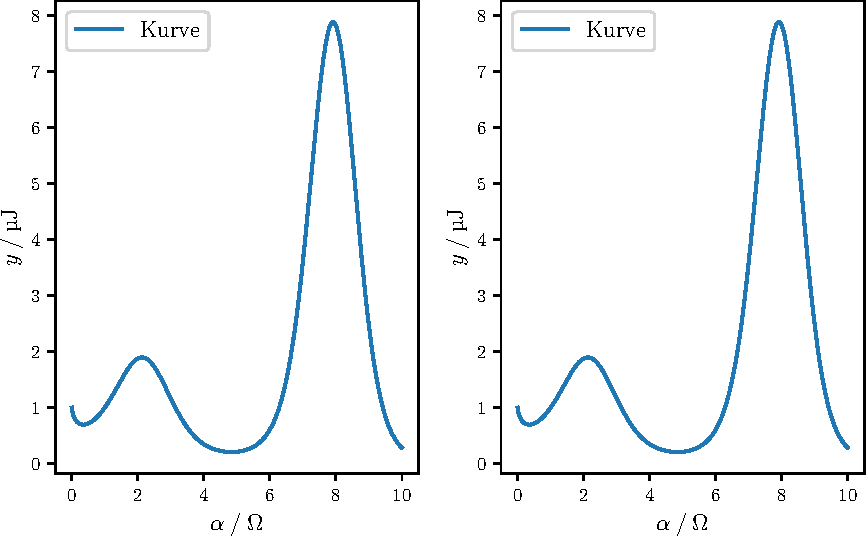
\includegraphics{plots/plot.pdf}
  \caption{Plot.}
  \label{fig:plot}
\end{figure}
%------

%Tabelle einbinden
\begin{table}
  \centering
  \caption{Beschreibung}
  \label{tab:Beispiel}
  \begin{tabular}{S[table-format=2.0] S[table-format=2.2]}
    \toprule
    {$f \:/\: \si{\kilo\hertz}$} & {$U_C \:/\: \si{\volt}$}\\
    \midrule
50  & 4.08\\
52  & 3.76\\
  \end{tabular}
\end{table}

\section{Diskussion}
\label{sec:Diskussion}
%relative Abweichung
Die relative Abweichung der Ergebnisse ergibt sich über
\begin{equation}\label{eqn:abweichung}
  \symup{\Delta}x = \frac{x_{\text{Messung}} - x_{\text{Theorie}}}{x_{\text{Theorie}}}.
\end{equation}
%-----------


\printbibliography{}

\end{document}
